\documentclass[11pt,a4paper]{article}

\usepackage{datetime}
\usepackage{graphicx}
\usepackage{subcaption}

\usepackage{hyperref}

\hypersetup{
    colorlinks=true,
    linkcolor=blue,
    filecolor=magenta,      
    urlcolor=cyan,
}


\title{Chapter 1 Lab Work: Overview of Distributed Systems}
\newdate{date}{15}{03}{2020}
\date{\displaydate{date}}
\author{Nguyen Ngoc Lam}

\begin{document}
 	\pagenumbering{gobble}
  	\maketitle
  	\newpage
  	\pagenumbering{arabic}
  	\tableofcontents
  	\newpage
	
	\section{Path of the html File That Contains the Content of the Default Website Apache}
	You can find it at (on linux): /var/www/html/
	\section{Default Port on Which Webserver Is Listening}
	The default port is 80. But you can change it in /etc/apache2/ports.conf (remember to switch to superuser first)
	\begin{figure}[h!]
  		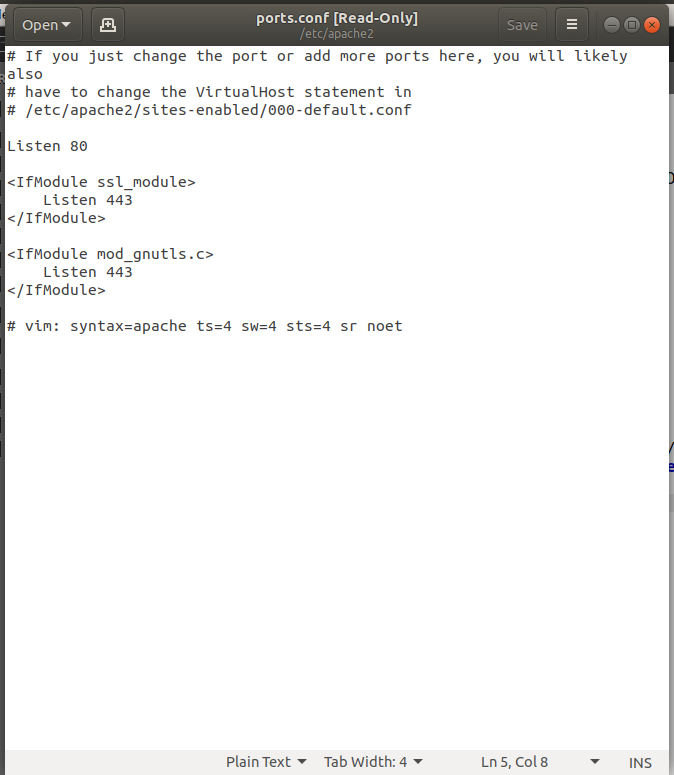
\includegraphics[width=\linewidth]{apache-default-port.png}
  		\caption{Apache port configuration file.}
  		\label{fig:apacheconf}
	\end{figure}
	\newpage
	\section{Meaning of Permission 755}
	\begin{tabular}{|c|c|c|c|}
	\hline 
	• & Write & Execute & Read \\ 
	\hline 
	Value & r & w & x \\ 
	\hline 
	Value (in number) & 4 & 2 & 1 \\ 
	\hline 
	\end{tabular} 
	\\Chmod 755 (chmod a+rwx,g-w,o-w) sets permissions so that, (U)ser / owner can read, can write and can execute. (G)roup can read, can't write and can execute. (O)thers can read, can't write and can execute.
	\section{Result of typing 2 addresses}
	When typing those two addresses, we will have:
	\begin{figure}[h!]
		\centering
  		\begin{subfigure}[b]{0.4\linewidth}
    		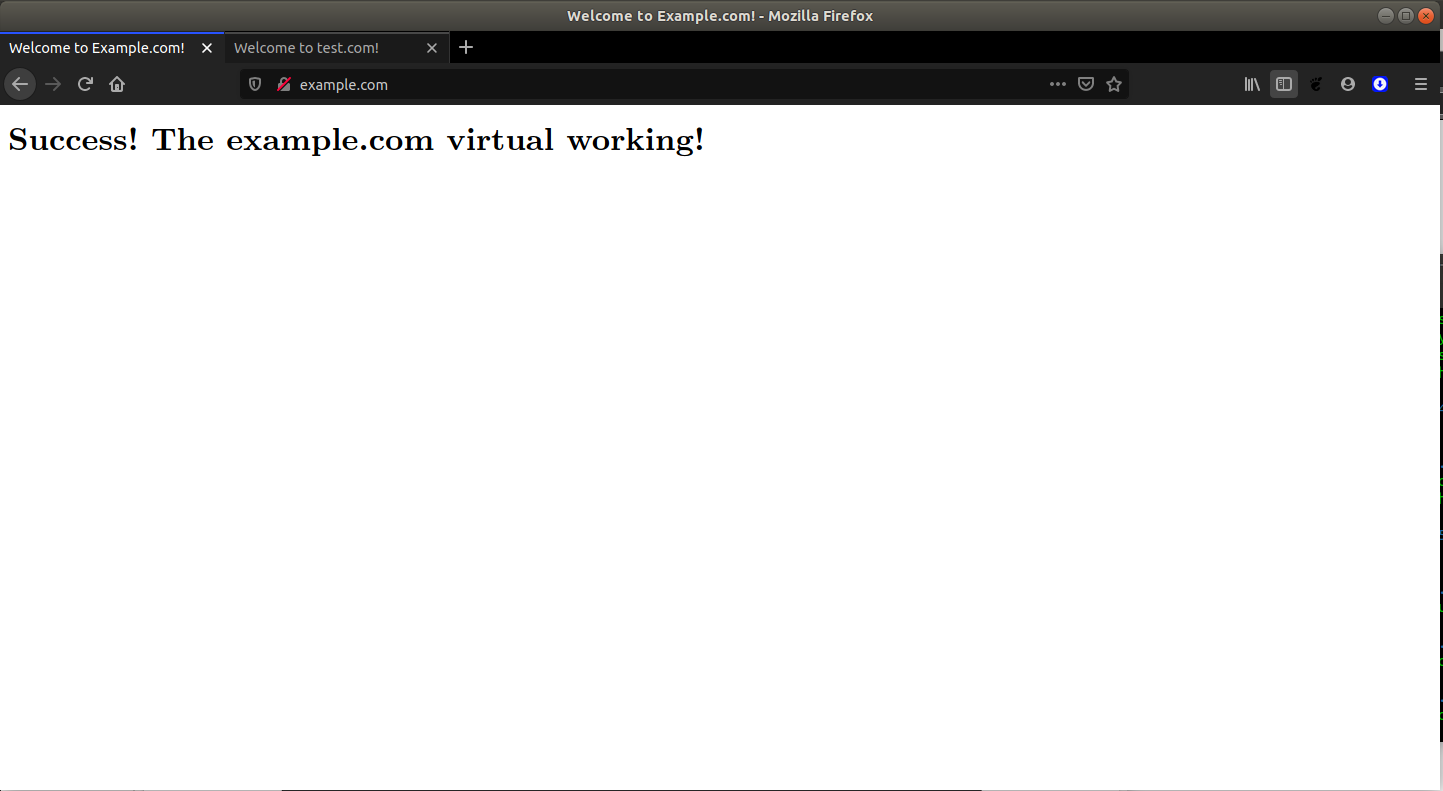
\includegraphics[width=\linewidth]{example-res.png}
    		\caption{When typing example.com}
  		\end{subfigure}
  		\begin{subfigure}[b]{0.4\linewidth}
    		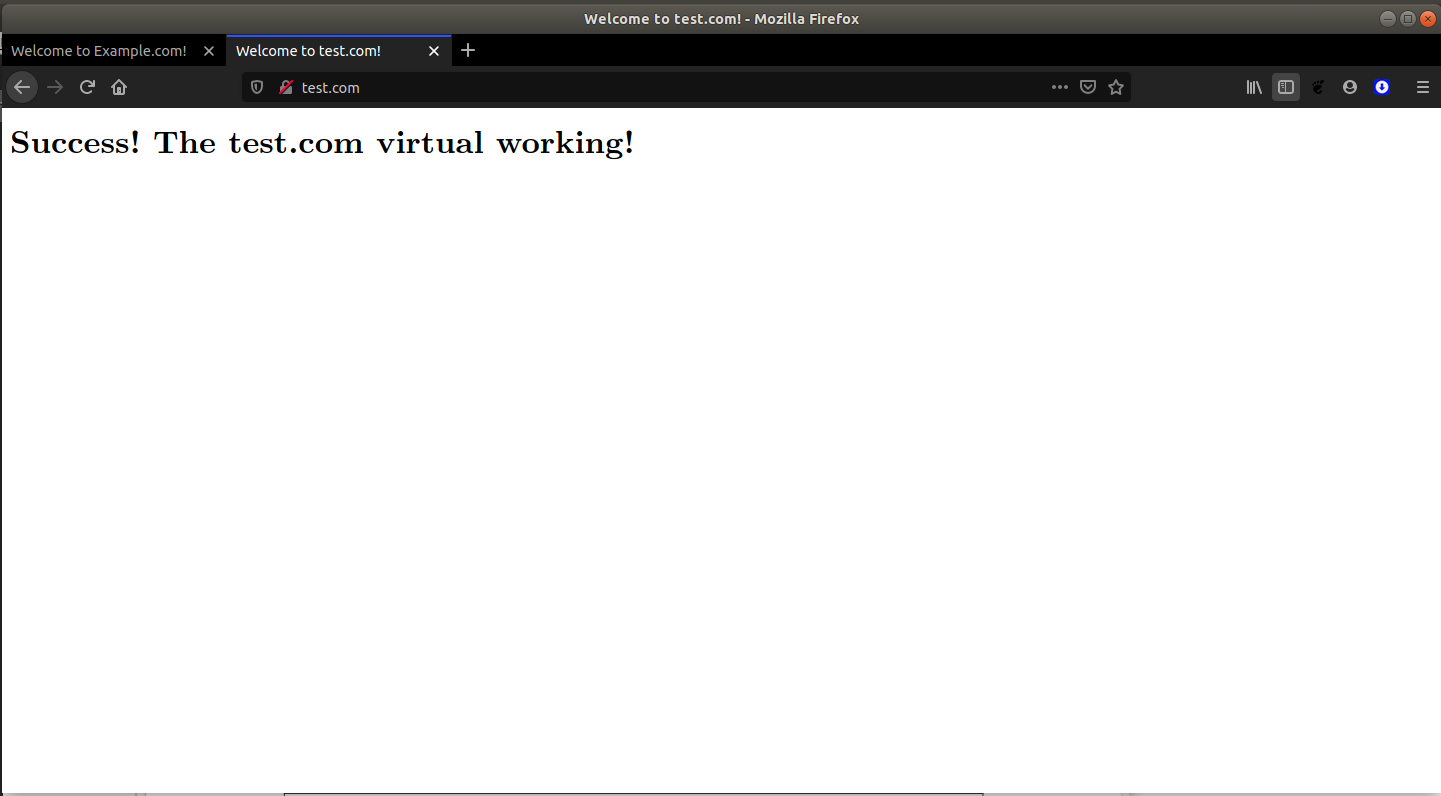
\includegraphics[width=\linewidth]{test-res.png}
    		\caption{When typing test.com}
  		\end{subfigure}
  		\caption{Result from web browser}
  		\label{fig:webbrowserres}
	\end{figure}
	\\Explain:\\
	When you ran two a2ensite commands for the two conf files, it will enable those two sites, which contained the information stored on the two html files above. After you reload apache to registered those changes and add the ip address (127.0.0.1 or localhost) and map it to the two websites.
	\\The results are showed above: when you type those 2 addresses to browser, it will show the html file.
	\section{Make others machine on LAN to connect to these two websites}
	\newpage
	\begin{enumerate}
		\item Type: "hostname -I" onto your terminal, you will see your local IP address (starting with 192.168.) and maybe a broadcast IP address of some other processes (like docker, if you installed) (starting with 172.). We only need the local IP address. We get the result like this:
		\begin{figure}[h!]
  			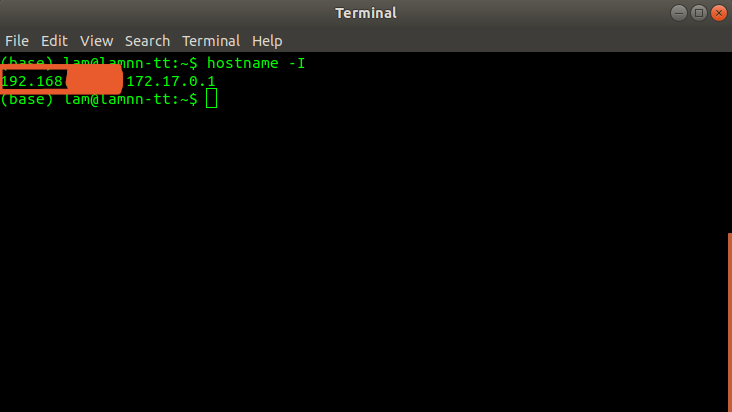
\includegraphics[width=\linewidth]{local-ip.png}
  			\caption{My local ip address}
  			\label{fig:loc-ip}
		\end{figure}
		\item On another computer on the same LAN, open the file /etc/hosts and add these lines with 192.168.x.x is the address you just obtained:\\
		"192.168.x.x example.com"\\
		"192.168.x.x test.com"
	\end{enumerate}
	\section{Code for the while loop}
	\begin{figure}[h!]
  		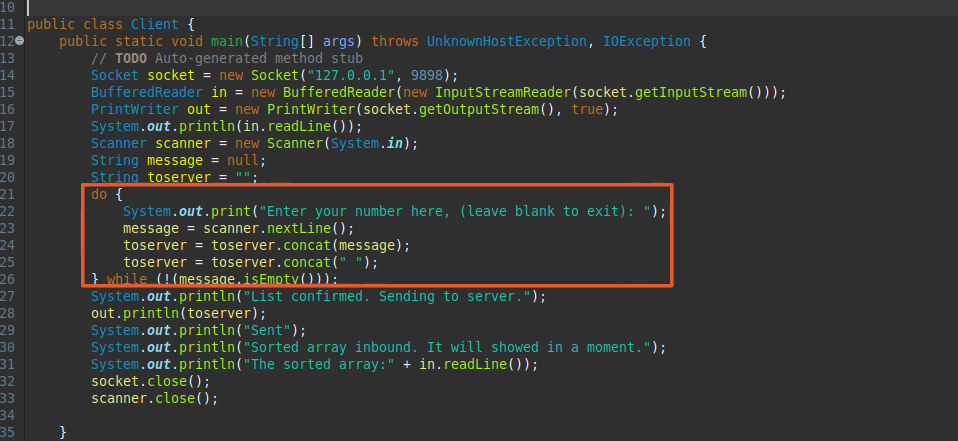
\includegraphics[width=\linewidth]{client-code.png}
  		\caption{My client-side}
  		\label{fig:client}
	\end{figure}
	\newpage
	\section{Role of method run()}
	\begin{itemize}
		\item Take the preprocessed input string from client-side.
		\item Split it in a string array.
		\item Parse each item in that array into integer, thus make an array of integer.
		\item Do the sort process (call class)
		\item Convert the integer array to String
		\item Send the result to Client and close socket.
	\end{itemize}
	\begin{figure}[h!]
  		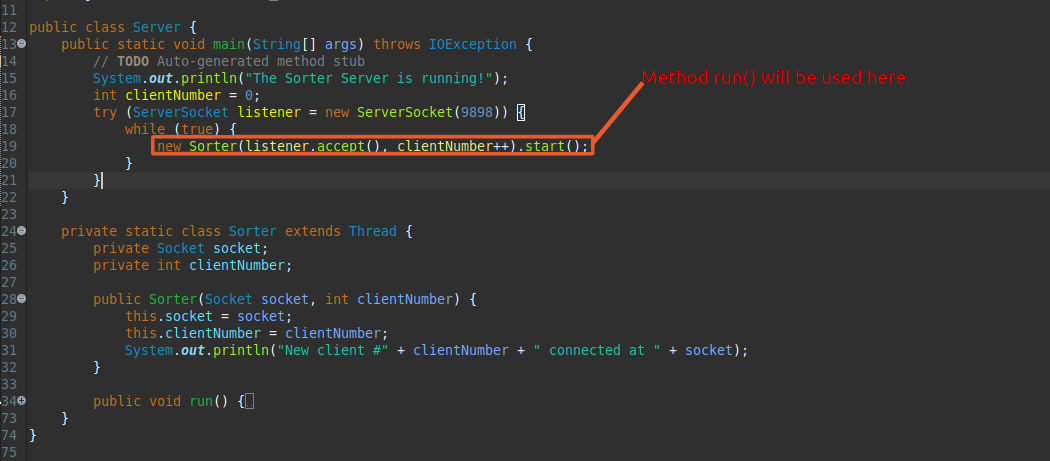
\includegraphics[width=\linewidth]{server-code.png}
  		\caption{My server side}
  		\label{fig:server}
	\end{figure}
	\section{Note}
	\begin{itemize}
		\item You can find my poject at: \href{https://github.com/lam1910/DistributedSystem}{Distributed System repository}
	\end{itemize}
\end{document}